%%%%%%%%%%%%%%%%%%%%% chapter.tex %%%%%%%%%%%%%%%%%%%%%%%%%%%%%%%%%
%
% sample chapter
%
% Use this file as a template for your own input.
%
%%%%%%%%%%%%%%%%%%%%%%%% Springer-Verlag %%%%%%%%%%%%%%%%%%%%%%%%%%
%\motto{Use the template \emph{chapter.tex} to style the various elements of your chapter content.}

\chapter{Rosetta Code Tasks starting with H}

\section*{HTTP}

Access and print a
\href{http://en.wikipedia.org/wiki/Uniform\_Resource\_Locator}{URL's}
content (the located resource) to the console. There is a separate
task for \emph{HTTPS Requests}.


\begin{wideverbatim}

(load "@lib/http.l")

(client "rosettacode.org" 80 NIL       # Connect to rosettacode
   (out NIL (echo)) )                  # Echo to standard output

\end{wideverbatim}

\pagebreak{}
\section*{HTTPS}

Print an HTTPS URL's content to the console. Checking the host
certificate for validity is recommended. The client should not
authenticate itself to the server --- the webpage
\href{https://sourceforge.net/}{https://sourceforge.net/} supports that
access policy --- as that is the subject of other
\emph{tasks}.

Readers may wish to contrast with the \emph{HTTP Request} task, and
also the task on \emph{HTTPS request with authentication}.


\begin{wideverbatim}

PicoLisp has no functionality for communicating with a HTTPS server (only for
the other direction), but it is easy to use an external tool

(in '(curl "https://sourceforge.net")  # Open a pipe to 'curl'
   (out NIL (echo)) )                  # Echo to standard output

\end{wideverbatim}

\pagebreak{}
\section*{HTTPS/Authenticated}

The goal of this task is to demonstrate \emph{HTTPS requests} with
authentication. Implementations of this task should not use client
certificates for this: that is the subject of \emph{another task}.

\begin{wideverbatim}

(let (User "Bill"  Pass "T0p5ecRet"  Url "https://www.example.com")
   (in (list 'curl "-u" (pack User ': Pass) Url)
      (while (line)
         (doSomeProcessingWithLine @) ) ) )

\end{wideverbatim}

\pagebreak{}
\section*{HTTPS/Client-authenticated}

Demonstrate how to connect to a web server over HTTPS where that
server requires that the client present a certificate to prove who
(s)he is. Unlike with the \emph{HTTPS request with authentication}
task, it is \emph{not} acceptable to perform the authentication by a
username/password or a set cookie.

This task is in general useful for use with \emph{webservice clients}
as it offers a high level of assurance that the client is an
acceptable counterparty for the server. For example,
\href{http://aws.amazon.com/}{Amazon Web Services} uses this style of
authentication.

\begin{wideverbatim}

(in '(curl "-E" "myCert.pem" "https://www.example.com")
   (while (line)
      (doSomeProcessingWithLine @) ) )

\end{wideverbatim}

\pagebreak{}
\section*{Hailstone sequence}

The Hailstone sequence of numbers can be generated from a starting
positive integer, n by:

\begin{itemize}
\item
  If n is 1 then the sequence ends.
\item
  If n is even then the next n of the sequence \texttt{= n/2}
\item
  If n is odd then the next n of the sequence \texttt{= (3 * n) + 1}
\end{itemize}

The (unproven),
\href{http://en.wikipedia.org/wiki/Collatz\_conjecture}{Collatz
  conjecture} is that the hailstone sequence for any starting number
always terminates.

\textbf{Task Description:}

\begin{enumerate}
\item
  Create a routine to generate the hailstone sequence for a number.
\item
  Use the routine to show that the hailstone sequence for the number 27
  has 112 elements starting with \texttt{27, 82, 41, 124} and ending
  with \texttt{8, 4, 2, 1}
\item
  Show the number less than 100,000 which has the longest hailstone
  sequence together with that sequences length.\\ (But don't show the
  actual sequence)!
\end{enumerate}

\textbf{See Also:}

\begin{itemize}
\item
  \href{http://xkcd.com/710}{xkcd} (humourous).
\end{itemize}

\begin{wideverbatim}

(de hailstone (N)
   (make
      (until (= 1 (link N))
         (setq N
            (if (bit? 1 N)
               (inc (* N 3))
               (/ N 2) ) ) ) ) )

(let L (hailstone 27)
   (println 27 (length L) (head 4 L) '- (tail 4 L)) )

(let N (maxi '((N) (length (hailstone N))) (range 1 100000))
   (println N (length (hailstone N))) )

Output:

27 112 (27 82 41 124) - (8 4 2 1)
77031 351

\end{wideverbatim}

\pagebreak{}
\section*{Hamming numbers}

\href{http://en.wikipedia.org/wiki/Hamming\_numbers\#Algorithms}{Hamming
numbers} are numbers of the form


\includegraphics[scale=.6]{graphics/27c40c22beaf5d82e9aabf41eb7d92a2.png}.

Hamming numbers are also known as ugly numbers and also 5-smooth numbers
(numbers whose prime divisors are less or equal to 5).

Generate the sequence of Hamming numbers, \emph{in increasing order}. In
particular:

\begin{enumerate}
\item
  Show the first twenty Hamming numbers.
\item
  Show the 1691st Hamming number (the last one below
  2\textsuperscript{31}).
\item
  Show the one millionth Hamming number (if the language -- or a
  convenient library -- supports arbitrary-precision integers).
\end{enumerate}

\textbf{References}

\begin{enumerate}
\item
  \href{http://en.wikipedia.org/wiki/Hamming\_numbers}{wp:Hamming\_numbers}
\item
  \href{http://en.wikipedia.org/wiki/Smooth\_number}{wp:Smooth\_number}
\item
  \href{http://dobbscodetalk.com/index.php?option=com\_content\&task=view\&id=913\&Itemid=85}{Hamming
  problem} from Dr. Dobb's CodeTalk (dead link as of Sep 2011; parts of
  the thread
  \href{http://drdobbs.com/blogs/architecture-and-design/228700538}{here}
  and
  \href{http://www.jsoftware.com/jwiki/Essays/Hamming\%20Number}{here}).
\end{enumerate}



\begin{wideverbatim}

(de hamming (N)
   (let (L (1)  H)
      (do N
         (for (X L X (cadr X))      # Find smallest result
            (setq H (car X)) )
         (idx 'L H NIL)             # Remove it
         (for I (2 3 5)             # Generate next results
            (idx 'L (* I H) T) ) )
      H ) )

(println (make (for N 20 (link (hamming N)))))
(println (hamming 1691))
(println (hamming 1000000))

Output:

(1 2 3 4 5 6 8 9 10 12 15 16 18 20 24 25 27 30 32 36)
2125764000
519312780448388736089589843750000000000000000000000000000000000000000000000000000000
# (took almost 2 hours)

\end{wideverbatim}

\pagebreak{}
\section*{Handle a signal}

Most general purpose operating systems provide interrupt facilities,
sometimes called signals. Unhandled signals generally terminate a
program in a disorderly manner. Signal handlers are created so that the
program behaves in a well-defined manner upon receipt of a signal.

For this task you will provide a program that displays a single integer
on each line of output at the rate of one integer in each half second.
Upon receipt of the SigInt signal (often created by the user typing
ctrl-C) the program will cease printing integers to its output, print
the number of seconds the program has run, and then the program will
terminate.

\begin{wideverbatim}

Put the following into a file, set it to executable, and run it

#!/usr/bin/picolisp /usr/lib/picolisp/lib.l

(push '*Bye '(println (*/ (usec) 1000000)) '(prinl))

(let Cnt 0
   (loop
      (println (inc 'Cnt))
      (wait 500) ) )

\end{wideverbatim}

\pagebreak{}
\section*{Happy numbers}

From Wikipedia, the free encyclopedia:

A \href{http://en.wikipedia.org/wiki/Happy\_number}{happy number} is
defined by the following process. Starting with any positive integer,
replace the number by the sum of the squares of its digits, and repeat
the process until the number equals 1 (where it will stay), or it loops
endlessly in a cycle which does not include 1. Those numbers for which
this process ends in 1 are happy numbers, while those that do not end in
1 are unhappy numbers. Display an example of your output here.

\textbf{Task:} Find and print the first 8 happy numbers.

See also: \href{http://oeis.org/A007770}{The happy numbers on OEIS}

\begin{wideverbatim}

(de happy? (N)
   (let Seen NIL
      (loop
         (T (= N 1) T)
         (T (member N Seen))
         (setq N
            (sum '((C) (** (format C) 2))
               (chop (push 'Seen N)) ) ) ) ) )

(let H 0
   (do 8
      (until (happy? (inc 'H)))
      (printsp H) ) )

Output:

1 7 10 13 19 23 28 31

\end{wideverbatim}

\pagebreak{}
\section*{Hash from two arrays}

Using two Arrays of equal length, create a Hash object where the
elements from one array (the keys) are linked to the elements of the
other (the values)

\begin{wideverbatim}

(let (Keys '(one two three)  Values (1 2 3))
   (mapc println
      (mapcar cons Keys Values) ) )

Output:

(one . 1)
(two . 2)
(three . 3)

\end{wideverbatim}

\pagebreak{}
\section*{Haversine formula}

The \textbf{haversine formula} is an equation important in navigation,
giving great-circle distances between two points on a sphere from their
longitudes and latitudes. It is a special case of a more general formula
in spherical trigonometry, the \textbf{law of haversines}, relating the
sides and angles of spherical ``triangles''.

\textbf{Task:} Implement a great-circle distance function, or use a
library function, to show the great-circle distance between Nashville
International Airport (BNA) in Nashville, TN, USA: N 36°7.2', W 86°40.2'
(36.12, -86.67) and Los Angeles International Airport (LAX) in Los
Angeles, CA, USA: N 33°56.4', W 118°24.0' (33.94, -118.40).

\begin{wideverbatim}

(scl 12)
(load "@lib/math.l")

(de haversine (Th1 Ph1 Th2 Ph2)
   (setq
      Ph1 (*/ (- Ph1 Ph2) pi 180.0)
      Th1 (*/ Th1 pi 180.0)
      Th2 (*/ Th2 pi 180.0) )
   (let
      (DX (- (*/ (cos Ph1) (cos Th1) 1.0) (cos Th2))
         DY (*/ (sin Ph1) (cos Th1) 1.0)
         DZ (- (sin Th1) (sin Th2)) )
      (* `(* 2 6371)
         (asin
            (/
               (sqrt (+ (* DX DX) (* DY DY) (* DZ DZ)))
               2 ) ) ) ) )

Test:

(prinl
   "Haversine distance: "
   (round (haversine 36.12 -86.67 33.94 -118.4))
   " km" )

Output:

Haversine distance: 2,886.444 km

\end{wideverbatim}

\pagebreak{}
\section*{Hello world/Graphical}

In this User Output task, the goal is to display the string ``Goodbye,
World!'' on a \emph{GUI} object (alert box, plain window, text area,
etc.).

See also: \emph{Hello world/Text}

\begin{wideverbatim}

(call 'dialog "--msgbox" "Goodbye, World!" 5 20)

\end{wideverbatim}

\pagebreak{}
\section*{Hello world/Line printer}

Cause a line printer attached to the computer to print a line containing
the message \texttt{Hello World!}

\textbf{Note:} A line printer is not the same as standard output. A
\href{http://en.wikipedia.org/wiki/line\_printer}{line printer} was an
older-style printer which prints one line at a time to a continuous ream
of paper. With some systems, a line printer can be any device attached
to an appropriate port (such as a parallel port).

\begin{wideverbatim}

(out '(lpr "-P" "Printer01")
   (prinl "Hello world") )

\end{wideverbatim}

\pagebreak{}
\section*{Hello world/Newline omission}

Some languages automatically insert a newline after outputting a string,
unless measures are taken to prevent its output. The purpose of this
task is to output the string ``Goodbye, World!'' preventing a trailing
newline from occuring.

\textbf{See also}

\begin{itemize}
\item
  \emph{Hello world/Graphical}
\item
  \emph{Hello world/Line Printer}
\item
  \emph{Hello world/Standard error}

\begin{wideverbatim}

(prin "Goodbye, world")

\end{wideverbatim}

\pagebreak{}
\section*{Hello world/Standard error}

\textbf{Hello world/Standard error} is part of \emph{Short Circuit}'s
\textbf{\emph{Console
    Program Basics}} selection.

A common practice in computing is to send error messages to a
different output stream than \emph{normal text console messages}. The
normal messages print to what is called ``standard output'' or
``standard out''. The error messages print to ``standard error''. This
separation can be used to redirect error messages to a different place
than normal messages.

Show how to print a message to standard error by printing ``Goodbye,
World!'' on that stream.

\begin{wideverbatim}

(out 2 (prinl "Goodbye, World!"))

\end{wideverbatim}

\pagebreak{}
\section*{Hello world/Text}

\textbf{Hello world/Text} is part of \emph{Short Circuit}'s
\textbf{\emph{Console Program Basics}} selection.

In this User Output task, the goal is to display the string ``Goodbye,
World!'' {[}sic{]} on a text console.

\textbf{See also}

\begin{itemize}
\item \emph{Hello world/Graphical}
\item \emph{Hello world/Line Printer}
\item \emph{Hello world/Newline omission}
\item \emph{Hello world/Standard error}
\item \emph{Hello world/Web server}
\end{itemize}

\begin{wideverbatim}

(prinl "Goodbye, World!")

\end{wideverbatim}

\pagebreak{}
\section*{Hello world/Web server}

The browser is the new \emph{GUI}!

The task is to serve our standard text ``Goodbye, World!'' to
\href{http://localhost:8080/}{http://localhost:8080/} so that it can
be viewed with a web browser. The provided solution must start or
implement a server that accepts multiple client connections and serves
text as requested.

Note that starting a web browser or opening a new window with this URL
is not part of the task. Additionally, it is permissible to serve the
provided page as a plain text file (there is no requirement to serve
properly formatted \emph{HTML} here). The browser will generally do
the right thing with simple text like this.

\begin{wideverbatim}

Contents of the file "goodbye.l":

(html 0 "Bye" NIL NIL
   "Goodbye, World!" )

Start server:

\$ pil @lib/http.l @lib/xhtml.l -'server 8080 "goodbye.l"' -wait

\end{wideverbatim}

\pagebreak{}
\section*{Here document}

A here document (or ``heredoc'') is a way of specifying a text block,
preserving the line breaks, indentation and other whitespace within the
text. Depending on the language being used a here document is
constructed using a command followed by ``\textless{}\textless{}'' (or
some other symbol) followed by a token string. The text block will then
start on the next line, and will be followed by the chosen token at the
beginning of the following line, which is used to mark the end of the
textblock.

The task is to demonstrate the use of here documents within the
language.

\begin{wideverbatim}

We can use the '[http://software-lab.de/doc/refH.html#here here]' function:

(out "file.txt"                        # Write to "file.txt"
   (prinl "### This is before the text ###")
   (here "TEXT-END")
   (prinl "### This is after the text ###") )
"There must be some way out of here", said the joker to the thief
"There's too much confusion, I can't get no relief"
TEXT-END

(in "file.txt" (echo))                 # Show "file.txt"

Output:

### This is before the text ###
"There must be some way out of here", said the joker to the thief
"There's too much confusion, I can't get no relief"
### This is after the text ###

\end{wideverbatim}

\pagebreak{}
\section*{Higher-order functions}

Pass a function \emph{as an argument} to another function.

C.f. \emph{First-class functions}


\begin{wideverbatim}

: (de first (Fun)
   (Fun) )
-> first

: (de second ()
   "second" )
-> second

: (first second)
-> "second"

: (de add (A B)
   (+ A B) )
-> add

: (add 1 2)
-> 3

: (de call-it (Fun X Y)
   (Fun X Y) )
-> call-it

: (call-it add 1 2)
-> 3

: (mapcar inc (1 2 3 4 5))
-> (2 3 4 5 6)

: (mapcar + (1 2 3) (4 5 6))
-> (5 7 9)

:  (mapcar add (1 2 3) (4 5 6))
-> (5 7 9)

\end{wideverbatim}

\pagebreak{}
\section*{History variables}

\emph{Storing the history of objects in a program is a common task.
Maintaining the history of an object in a program has traditionally
required programmers either to write specific code for handling the
historical data, or to use a library which supports history logging.}

\emph{History variables are variables in a programming language which
store not only their current value, but also the values they have
contained in the past. Some existing languages do provide support for
history variables. However these languages typically have many limits
and restrictions on use of history variables.} \emph{}

\href{http://www.bod.com/index.php?id=3435\&objk\_id=148050}{``History
Variables: The Semantics, Formal Correctness, and Implementation of
History Variables in an Imperative Programming Language'' by Mallon and
Takaoka}

Concept also discussed on
\href{http://lambda-the-ultimate.org/node/3111}{LtU} and
\href{http://www.patents.com/us-7111283.html}{Patents.com}.

\begin{description}
\item[Task]
\end{description}

Demonstrate History variable support:

\begin{itemize}
\item
  enable history variable support (if needed)
\item
  define a history variable
\item
  assign three values
\item
  non-destructively display the history
\item
  recall the three values.
\end{itemize}

For extra points, if the language of choice does not support history
variables, demonstrate how this might be implemented.


\begin{wideverbatim}

(de setH ("Var" Val)
   (when (val "Var")
      (with "Var"
         (=: history (cons @ (: history))) ) )
   (set "Var" Val) )

(de restoreH ("Var")
   (set "Var" (pop (prop "Var" 'history))) )

Test:

: (setH 'A "Hello world")
-> "Hello world"

: (setH 'A '(a b c d))
-> (a b c d)

: (setH 'A 123)
-> 123

: A
-> 123

: (get 'A 'history)
-> ((a b c d) "Hello world")

: (restoreH 'A)
-> (a b c d)

: (restoreH 'A)
-> "Hello world"

: A
-> "Hello world"

: (restoreH 'A)
-> NIL

\end{wideverbatim}

\pagebreak{}
\section*{Hofstadter Figure-Figure sequences}

These two sequences of positive integers are defined as:

\begin{figure}[H]
\centering
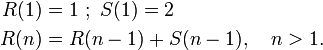
\includegraphics[scale=.6]{graphics/8b92ddffc196683c9c4b2fb5f6f91d7c.png}
% \caption{\textbackslash{}begin\{align\}
% R(1)\&=1\textbackslash{}~;\textbackslash{} S(1)=2
% \textbackslash{}\textbackslash{} R(n)\&=R(n-1)+S(n-1),
% \textbackslash{}quad n\textgreater{}1. \textbackslash{}end\{align\}}
\end{figure}

The sequence \emph{S}(\emph{n}) is further defined as the sequence of
positive integers \emph{not} present in \emph{R}(\emph{n}).

Sequence R starts: 1, 3, 7, 12, 18, \ldots{}

Sequence S starts: 2, 4, 5, 6, 8, \ldots{}

Task:

\begin{enumerate}
\item
  Create two functions named ffr and ffs that when given n return R(n)
  or S(n) respectively.\\(Note that R(1) = 1 and S(1) = 2 to avoid
  off-by-one errors).
\item
  No maximum value for n should be assumed.
\item
  Calculate and show that the first ten values of R are: 1, 3, 7, 12,
  18, 26, 35, 45, 56, and 69
\item
  Calculate and show that the first 40 values of ffr plus the first 960
  values of ffs include all the integers from 1 to 1000 exactly once.
\end{enumerate}

\begin{description}
\item[References]
\end{description}

\begin{itemize}
\item
  Sloane's \href{http://oeis.org/A005228}{A005228} and
  \href{http://oeis.org/A030124}{A030124}.
\item
  \href{http://mathworld.wolfram.com/HofstadterFigure-FigureSequence.html}{Wolfram
  Mathworld}
\item
  Wikipedia:
  \href{http://en.wikipedia.org/wiki/Hofstadter\_sequence\#Hofstadter\_Figure-Figure\_sequences}{Hofstadter
  Figure-Figure sequences}.
\end{itemize}


\begin{wideverbatim}

(setq *RNext 2)

(de ffr (N)
   (cache '(NIL) (pack (char (hash N)) N)
      (if (= 1 N)
         1
         (+ (ffr (dec N)) (ffs (dec N))) ) ) )

(de ffs (N)
   (cache '(NIL) (pack (char (hash N)) N)
      (if (= 1 N)
         2
         (let S (inc (ffs (dec N)))
            (when (= S (ffr *RNext))
               (inc 'S)
               (inc '*RNext) )
            S ) ) ) )

Test:

: (mapcar ffr (range 1 10))
-> (1 3 7 12 18 26 35 45 56 69)

: (=
   (range 1 1000)
   (sort (conc (mapcar ffr (range 1 40)) (mapcar ffs (range 1 960)))) )
-> T

\end{wideverbatim}

\pagebreak{}
\section*{Hofstadter Q sequence}

The
\href{http://en.wikipedia.org/wiki/Hofstadter\_sequence\#Hofstadter\_Q\_sequence}{Hofstadter
Q sequence} is defined as:

\begin{figure}[H]
\centering
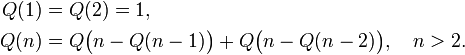
\includegraphics[scale=.6]{graphics/a049527fb76c4d324e8790190e84ba28.png}
% \caption{\textbackslash{}begin\{align\} Q(1)\&=Q(2)=1,
% \textbackslash{}\textbackslash{}
% Q(n)\&=Q\textbackslash{}big(n-Q(n-1)\textbackslash{}big)+Q\textbackslash{}big(n-Q(n-2)\textbackslash{}big),
% \textbackslash{}quad n\textgreater{}2. \textbackslash{}end\{align\}}
\end{figure}

It is defined like the \emph{Fibonacci sequence}, but whereas the next
term in the Fibonacci sequence is the sum of the previous two terms,
in the Q sequence the previous two terms tell you how far to go back
in the Q sequence to find the two numbers to sum to make the next term
of the sequence.

\begin{description}
\item[Task]
\end{description}

\begin{itemize}
\item
  Confirm and display that the first ten terms of the sequence are: 1,
  1, 2, 3, 3, 4, 5, 5, 6, and 6
\item
  Confirm and display that the 1000'th term is: 502
\end{itemize}

Optional extra credit

\begin{itemize}
\item
  Count and display how many times a member of the sequence is less than
  its preceding term for terms up to and including the 100,000'th term.
\item
  Ensure that the extra credit solution `safely' handles being initially
  asked for an n'th term where n is large.\\ (This point is to ensure
  that caching and/or recursion limits, if it is a concern, is correctly
  handled).
\end{itemize}


\begin{wideverbatim}

(de q (N)
   (cache '(NIL) (pack (char (hash N)) N)
      (if (>= 2 N)
         1
         (+
            (q (- N (q (dec N))))
            (q (- N (q (- N 2)))) ) ) ) )

Test:

: (mapcar q (range 1 10))
-> (1 1 2 3 3 4 5 5 6 6)

: (q 1000)
-> 502

: (let L (mapcar q (range 1 100000)) (!)
   (cnt < (cdr L) L) )
-> 49798

\end{wideverbatim}

\pagebreak{}
\section*{Hofstadter-Conway \$10,000 sequence}

The definition of the sequence is colloquially described as:

\begin{itemize}
\item
  Starting with the list {[}1,1{]},
\item
  Take the last number in the list so far: 1, I'll call it x.
\item
  Count forward x places from the beginning of the list to find the
  first number to add (1)
\item
  Count backward x places from the end of the list to find the second
  number to add (1)
\item
  Add the two indexed numbers from the list and the result becomes the
  next number in the list (1+1)
\item
  This would then produce {[}1,1,2{]} where 2 is the third element of
  the sequence.
\end{itemize}

Note that indexing for the description above starts from alternately the
left and right ends of the list and starts from an index of \emph{one}.

A less wordy description of the sequence is:

\begin{verbatim}
   a(1)=a(2)=1
   a(n)=a(a(n-1))+a(n-a(n-1))
\end{verbatim}

The sequence begins:

\begin{verbatim}
   1, 1, 2, 2, 3, 4, 4, 4, 5, ...
\end{verbatim}

Interesting features of the sequence are that:

\begin{itemize}
\item
  a(n)/n tends to 0.5 as n grows towards infinity.
\item
  a(n)/n where n is a power of 2 is 0.5
\item
  For n\textgreater{}4 the maximal value of a(n)/n between successive
  powers of 2 decreases.
\end{itemize}

\begin{figure}[H]
  \centering
   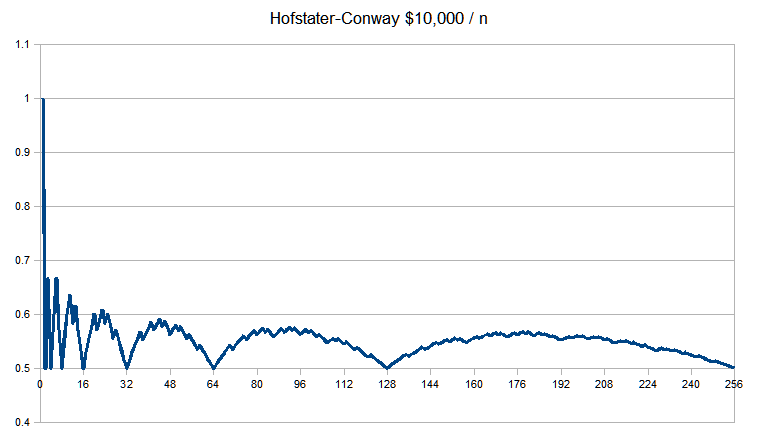
\includegraphics[scale=.6]{graphics/Hofstadter_conway_10K.png}  
\end{figure}

The sequence is so named because
\href{http://en.wikipedia.org/wiki/John\_Horton\_Conway}{John Conway}
\href{http://www.nytimes.com/1988/08/30/science/intellectual-duel-brash-challenge-swift-response.html}{offered
a prize} of \$10,000 to the first person who could find the first
position, p in the sequence where

\begin{verbatim}
   |a(n)/n| < 0.55 for all n > p.
\end{verbatim}

It was later found that
\href{http://en.wikipedia.org/wiki/Douglas\_Hofstadter}{Hofstadter} had
also done prior work on the sequence.

The `prize' was won quite quickly by
\href{http://www.research.avayalabs.com/gcm/usa/en-us/people/all/mallows.htm}{Dr.
Colin L. Mallows} who proved the properties of the sequence and allowed
him to find the value of n. (Which is much smaller than the
3,173,375,556. quoted in the NYT article)

\pagebreak{}
\textbf{The task is to:}

\begin{enumerate}
\item
  Create a routine to generate members of theH ofstadter-Conway \$10,000
  sequence.
\item
  Use it to show the maxima of a(n)/n between successive powers of two
  up to 2**20
\item
  As a stretch goal: Compute the value of n that would have won the
  prize and confirm it is true for n up to 2**20
\end{enumerate}

References:

\begin{itemize}
\item
  \href{http://www.jstor.org/stable/2324028}{Conways Challenge
  Sequence}, Mallows' own account.
\item
  \href{http://mathworld.wolfram.com/Hofstadter-Conway10000-DollarSequence.html}{Mathworld
  Article}.
\end{itemize}

\begin{wideverbatim}

(de hofcon (N)
   (cache '(NIL) (pack (char (hash N)) N)
      (if (>= 2 N)
         1
         (+
            (hofcon (hofcon (dec N)))
            (hofcon (- N (hofcon (dec N)))) ) ) ) )

(scl 20)

(de sequence (M)
   (let (Lim 4  Max 0  4k\$ 0)
      (for (N 3 (>= M N) (inc N))
         (let V (*/ (hofcon N) 1.0 N)
            (setq Max (max Max V))
            (when (>= V 0.55)
               (setq 4k\$ N) )
            (when (= N Lim)
               (prinl
                  "Maximum between " (/ Lim 2)
                  " and " Lim
                  " was " (format Max `*Scl) )
               (inc 'Lim Lim)
               (zero Max) ) ) )
      (prinl
         "Win with " (inc 4k\$)
         " (the task requests 'n >= p')" ) ) )

(sequence (** 2 20))

Output:

Maximum between 2 and 4 was 0.66666666666666666667
Maximum between 4 and 8 was 0.66666666666666666667
Maximum between 8 and 16 was 0.63636363636363636364
Maximum between 16 and 32 was 0.60869565217391304348
Maximum between 32 and 64 was 0.59090909090909090909
Maximum between 64 and 128 was 0.57608695652173913043
Maximum between 128 and 256 was 0.56741573033707865169
Maximum between 256 and 512 was 0.55945945945945945946
Maximum between 512 and 1024 was 0.55493741307371349096
Maximum between 1024 and 2048 was 0.55010087424344317418
Maximum between 2048 and 4096 was 0.54746289264756644805
Maximum between 4096 and 8192 was 0.54414474786396381303
Maximum between 8192 and 16384 was 0.54244270878036220067
Maximum between 16384 and 32768 was 0.54007109751158709445
Maximum between 32768 and 65536 was 0.53878402058425570614
Maximum between 65536 and 131072 was 0.53704365699986594575
Maximum between 131072 and 262144 was 0.53602006781156104419
Maximum between 262144 and 524288 was 0.53464543107811232092
Maximum between 524288 and 1048576 was 0.53377922996336783427
Win with 1490 (the task requests 'n >= p')

\end{wideverbatim}

\pagebreak{}
\section*{Holidays related to Easter}

Calculate the date of
\href{http://en.wikipedia.org/wiki/Easter}{Easter},
\href{http://en.wikipedia.org/wiki/Ascension\_Thursday}{Ascension
Thursday}, \href{http://en.wikipedia.org/wiki/Pentecost}{Pentecost},
\href{http://en.wikipedia.org/wiki/Trinity\_Sunday}{Trinity Sunday} \&
\href{http://en.wikipedia.org/wiki/Corpus\_Christi\_(feast)}{Corpus
Christi feast}.

As the example calculate for the first year of each century from 400 to
2100 \href{http://en.wikipedia.org/wiki/Common\_Era}{CE} and also for
years 2010 to 2020 CE.

Note: From year 325 CE on,
\href{http://en.wikipedia.org/wiki/Easter\_Sunday}{Easter Sunday} is the
Sunday following the first
\href{http://en.wikipedia.org/wiki/Ecclesiastical\_full\_moon}{Ecclesiastical
full moon} not earlier than the equinox date in 325 --- 21 March. The
Ecclesiastical full moon does not always correspond to the astronomical
full moon since in 325 fine details of Lunar dynamics were not yet fully
understood.

\href{http://en.wikipedia.org/wiki/Metonic\_cycle}{Metonic cycle}:
Taking a year to be 1/19th of this 6940-day cycle gives a year length of
365~+~1/4~+~1/76 days (the unrounded cycle is much more accurate), which
is slightly more than 12 synodic months. To keep the 12-month lunar year
in pace with the solar year, an
\href{http://en.wikipedia.org/wiki/intercalary}{intercalary} 13th month
would have to be added on seven occasions during the nineteen-year
period. Meton introduced a formula for intercalation in circa~432~BC.


\begin{wideverbatim}

(load "@lib/cal.l")  # For 'easter' function

(de dayMon (Dat)
   (let D (date Dat)
      (list (day Dat *Day) " " (align 2 (caddr D)) " " (get *Mon (cadr D))) ) )

(for Y (append (range 400 2100 100) (range 2010 2020))
   (let E (easter Y)
      (prinl
         (align 4 Y)
         # E = Easter, A = Ascension, P = Pentecost, T = Trinity, C = Corpus
         " E: " (dayMon E)
         ", A: " (dayMon (+ E 39))
         ", P: " (dayMon (+ E 49))
         ", T: " (dayMon (+ E 56))
         ", C: " (dayMon (+ E 60)) ) ) )

\end{wideverbatim}

\begin{wideverbatim}

[E = Easter, A = Ascension, P = Pentecost, T = Trinity, C = Corpus]

Output:

 400 E: Sun  2 Apr, A: Thu 11 May, P: Sun 21 May, T: Sun 28 May, C: Thu  1 Jun
 500 E: Sun  4 Apr, A: Thu 13 May, P: Sun 23 May, T: Sun 30 May, C: Thu  3 Jun
 600 E: Sun 13 Apr, A: Thu 22 May, P: Sun  1 Jun, T: Sun  8 Jun, C: Thu 12 Jun
 700 E: Sun 15 Apr, A: Thu 24 May, P: Sun  3 Jun, T: Sun 10 Jun, C: Thu 14 Jun
 800 E: Sun 23 Apr, A: Thu  1 Jun, P: Sun 11 Jun, T: Sun 18 Jun, C: Thu 22 Jun
 900 E: Sun 28 Mar, A: Thu  6 May, P: Sun 16 May, T: Sun 23 May, C: Thu 27 May
1000 E: Sun 30 Mar, A: Thu  8 May, P: Sun 18 May, T: Sun 25 May, C: Thu 29 May
1100 E: Sun  8 Apr, A: Thu 17 May, P: Sun 27 May, T: Sun  3 Jun, C: Thu  7 Jun
1200 E: Sun  9 Apr, A: Thu 18 May, P: Sun 28 May, T: Sun  4 Jun, C: Thu  8 Jun
1300 E: Sun 18 Apr, A: Thu 27 May, P: Sun  6 Jun, T: Sun 13 Jun, C: Thu 17 Jun
1400 E: Sun 20 Apr, A: Thu 29 May, P: Sun  8 Jun, T: Sun 15 Jun, C: Thu 19 Jun
1500 E: Sun  1 Apr, A: Thu 10 May, P: Sun 20 May, T: Sun 27 May, C: Thu 31 May
1600 E: Sun  2 Apr, A: Thu 11 May, P: Sun 21 May, T: Sun 28 May, C: Thu  1 Jun
1700 E: Sun 11 Apr, A: Thu 20 May, P: Sun 30 May, T: Sun  6 Jun, C: Thu 10 Jun
1800 E: Sun 13 Apr, A: Thu 22 May, P: Sun  1 Jun, T: Sun  8 Jun, C: Thu 12 Jun
1900 E: Sun 15 Apr, A: Thu 24 May, P: Sun  3 Jun, T: Sun 10 Jun, C: Thu 14 Jun
2000 E: Sun 23 Apr, A: Thu  1 Jun, P: Sun 11 Jun, T: Sun 18 Jun, C: Thu 22 Jun
2100 E: Sun 28 Mar, A: Thu  6 May, P: Sun 16 May, T: Sun 23 May, C: Thu 27 May
2010 E: Sun  4 Apr, A: Thu 13 May, P: Sun 23 May, T: Sun 30 May, C: Thu  3 Jun
2011 E: Sun 24 Apr, A: Thu  2 Jun, P: Sun 12 Jun, T: Sun 19 Jun, C: Thu 23 Jun
2012 E: Sun  8 Apr, A: Thu 17 May, P: Sun 27 May, T: Sun  3 Jun, C: Thu  7 Jun
2013 E: Sun 31 Mar, A: Thu  9 May, P: Sun 19 May, T: Sun 26 May, C: Thu 30 May
2014 E: Sun 20 Apr, A: Thu 29 May, P: Sun  8 Jun, T: Sun 15 Jun, C: Thu 19 Jun
2015 E: Sun  5 Apr, A: Thu 14 May, P: Sun 24 May, T: Sun 31 May, C: Thu  4 Jun
2016 E: Sun 27 Mar, A: Thu  5 May, P: Sun 15 May, T: Sun 22 May, C: Thu 26 May
2017 E: Sun 16 Apr, A: Thu 25 May, P: Sun  4 Jun, T: Sun 11 Jun, C: Thu 15 Jun
2018 E: Sun  1 Apr, A: Thu 10 May, P: Sun 20 May, T: Sun 27 May, C: Thu 31 May
2019 E: Sun 21 Apr, A: Thu 30 May, P: Sun  9 Jun, T: Sun 16 Jun, C: Thu 20 Jun
2020 E: Sun 12 Apr, A: Thu 21 May, P: Sun 31 May, T: Sun  7 Jun, C: Thu 11 Jun

\end{wideverbatim}

\pagebreak{}
\section*{Horizontal sundial calculations}

A program that calculates the hour, sun hour angle, dial hour line angle
from 6am to 6pm for an \emph{operator} entered location.

As the example the user is prompted for a location and inputs the
latitude and longitude 4°57′S 150°30′W (4.95°S 150.5°W) of
\href{http://en.wikipedia.org/wiki/Jules\_Verne}{Jules Verne}'s
\emph{\href{http://en.wikipedia.org/wiki/The\_Mysterious\_Island}{Lincoln
Island}}, aka
\emph{\href{http://en.wikipedia.org/wiki/Ernest\_Legouve\_Reef}{Ernest
Legouve Reef})}. With a legal meridian of 150°W.

Wikipedia: A \href{http://en.wikipedia.org/wiki/sundial}{sundial} is a
device that measures time by the position of the
\href{http://en.wikipedia.org/wiki/Sun}{Sun}. In common designs such as
the horizontal sundial, the sun casts a
\href{http://en.wikipedia.org/wiki/shadow}{shadow} from its \emph{style}
(also called its \href{http://en.wikipedia.org/wiki/Gnomon}{Gnomon}, a
thin rod or a sharp, straight edge) onto a flat surface marked with
lines indicating the hours of the day. As the sun moves across the sky,
the shadow-edge progressively aligns with different hour-lines on the
plate. Such designs rely on the style being aligned with the axis of the
Earth's rotation. Hence, if such a sundial is to tell the correct time,
the style must point towards
\href{http://en.wikipedia.org/wiki/true\_north}{true north} (not the
\href{http://en.wikipedia.org/wiki/North\_Magnetic\_Pole}{north} or
\href{http://en.wikipedia.org/wiki/Magnetic\_South\_Pole}{south magnetic
pole}) and the style's angle with horizontal must equal the sundial's
geographical \href{http://en.wikipedia.org/wiki/latitude}{latitude}.

\begin{wideverbatim}

(load "@lib/math.l")

(de prompt (Str . Arg)
   (prin Str " => ")
   (set (car Arg) (in NIL (read))) )

(use (Lat Lng Ref)
   (prompt "Enter latitude      " Lat)
   (prompt "Enter longitude     " Lng)
   (prompt "Enter legal meridian" Ref)
   (prinl)
   (let Slat (sin (*/ Lat pi 180.0))
      (prinl "    sine of latitude:   " (round Slat))
      (prinl "    diff longitude:     " (round (- Lng Ref)))
      (prinl)
      (prinl "Hour, sun hour angle, dial hour line angle from 6am to 6pm")
      (for H (range -6 6)
         (let Hra (- (* 15.0 H) (- Lng Ref))
            (let Hla (*/ (atan (*/ Slat (tan (*/ Hra pi 180.0)) 1.0)) 180.0 pi)
               (prinl
                  "HR="
                  (align 3 H)
                  "; HRA="
                  (align 8 (round Hra))
                  "; HLA="
                  (align 8 (round Hla)) ) ) ) ) ) )

Output:

Enter latitude       => -4.95
Enter longitude      => -150.5
Enter legal meridian => -150.          # Don't omit the '.' here

    sine of latitude:   -0.086
    diff longitude:     -0.500

Hour, sun hour angle, dial hour line angle from 6am to 6pm
HR= -6; HRA= -89.500; HLA=  84.225
HR= -5; HRA= -74.500; HLA=  17.283
HR= -4; HRA= -59.500; HLA=   8.334
HR= -3; HRA= -44.500; HLA=   4.847
HR= -2; HRA= -29.500; HLA=   2.795
HR= -1; HRA= -14.500; HLA=   1.278
HR=  0; HRA=   0.500; HLA=  -0.043
HR=  1; HRA=  15.500; HLA=  -1.371
HR=  2; HRA=  30.500; HLA=  -2.910
HR=  3; HRA=  45.500; HLA=  -5.018
HR=  4; HRA=  60.500; HLA=  -8.671
HR=  5; HRA=  75.500; HLA= -18.451
HR=  6; HRA=  90.500; HLA=  84.225

\end{wideverbatim}

\pagebreak{}
\section*{Horner's rule for polynomial evaluation}

A fast scheme for evaluating a polynomial such as:

\begin{figure}[H]
\centering
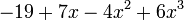
\includegraphics[scale=.6]{graphics/9eb10505118ec312428f2a4fb8b05d1f.png}
% \caption{-19+7x-4x\^{}2+6x\^{}3\textbackslash{},}
\end{figure}

when

\begin{figure}[H]
\centering
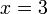
\includegraphics[scale=.6]{graphics/2663fd4ac67a9a044457d845268cd7ce.png}
\end{figure}

is to arrange the computation as follows:

\begin{figure}[H]
\centering

\includegraphics[scale=.6]{graphics/f1267a46eea12e7c046cfc7fcb859cc2.png}
% \caption{((((0) x + 6) x + (-4)) x + 7) x + (-19)\textbackslash{};}
\end{figure}

And compute the result from the innermost brackets outwards as in this
pseudocode:

\begin{verbatim}
coefficients := [-19, 7, -4, 6] # list coefficients of all x^0..x^n in order
x := 3
accumulator := 0
for i in length(coefficients) downto 1 do
    # Assumes 1-based indexing for arrays
    accumulator := ( accumulator * x ) + coefficients[i]
done
# accumulator now has the answer
\end{verbatim}

\textbf{Task Description}

Create a routine that takes a list of coefficients of a polynomial in
order of increasing powers of x; together with a value of x to compute
its value at, and return the value of the polynomial at that value using
\href{http://www.physics.utah.edu/~detar/lessons/c++/array/node1.html}{Horner's
rule}.

Cf. \emph{Formal power series}


\begin{wideverbatim}

(de horner (Coeffs X)
   (let Res 0
      (for C (reverse Coeffs)
         (setq Res (+ C (* X Res))) ) ) )

: (horner (-19.0 7.0 -4.0 6.0) 3.0)
-> 128

\end{wideverbatim}

\pagebreak{}
\section*{Host introspection}

Print the
\href{http://en.wikipedia.org/wiki/Word\_size\#Word\_size\_choice}{word
size} and \href{http://en.wikipedia.org/wiki/Endianness}{endianness} of
the host machine.

See also: \emph{Variable size/Get}


\begin{wideverbatim}

(in (cmd)                              # Inspect ELF header
   (rd 4)                              # Skip "7F" and 'E', 'L' and 'F'
   (prinl
      (case (rd 1)                     # Get EI_CLASS byte
         (1 "32 bits")
         (2 "64 bits")
         (T "Bad EI_CLASS") ) )
   (prinl
      (case (rd 1)                     # Get EI_DATA byte
         (1 "Little endian")
         (2 "Big endian")
         (T "Bad EI_DATA") ) ) )

\end{wideverbatim}

\pagebreak{}
\section*{Hostname}

Find the name of the host on which the routine is running.

\begin{wideverbatim}

This will just print the hostname:

(call 'hostname)

To use it as a string in a program:

(in '(hostname) (line T))

\end{wideverbatim}

\pagebreak{}
\section*{Huffman coding}

Huffman encoding is a way to assign binary codes to symbols that reduces
the overall number of bits used to encode a typical string of those
symbols.

For example, if you use letters as symbols and have details of the
frequency of occurrence of those letters in typical strings, then you
could just encode each letter with a fixed number of bits, such as in
ASCII codes. You can do better than this by encoding more frequently
occurring letters such as e and a, with smaller bit strings; and less
frequently occurring letters such as q and x with longer bit strings.

Any string of letters will be encoded as a string of bits that are
no-longer of the same length per letter. To successfully decode such as
string, the smaller codes assigned to letters such as `e' cannot occur
as a prefix in the larger codes such as that for `x'.

If you were to assign a code 01 for `e' and code 011 for `x', then if
the bits to decode started as 011\ldots{} then you would not know if you
should decode an `e' or an `x'.

The Huffman coding scheme takes each symbol and its weight (or frequency
of occurrence), and generates proper encodings for each symbol taking
account of the weights of each symbol, so that higher weighted symbols
have less bits in their encoding. (See the
\href{http://en.wikipedia.org/wiki/Huffman\_coding}{WP article} for more
information).

A Huffman encoding can be computed by first creating a tree of nodes:

\begin{figure}[H]
\centering
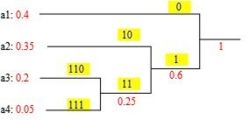
\includegraphics[scale=.6]{graphics/250px-Huffman_coding_example.jpg}
\end{figure}


\begin{enumerate}
\item
  Create a leaf node for each symbol and add it to the
  \emph{priority queue}.
\item
  While there is more than one node in the queue:

  \begin{enumerate}
  \item
    Remove the node of highest priority (lowest probability) twice to
    get two nodes.
  \item
    Create a new internal node with these two nodes as children and with
    probability equal to the sum of the two nodes' probabilities.
  \item
    Add the new node to the queue.
  \end{enumerate}
\item
  The remaining node is the root node and the tree is complete.
\end{enumerate}

Traverse the constructed binary tree from root to leaves assigning and
accumulating a `0' for one branch and a `1' for the other at each node.
The accumulated zeros and ones at each leaf constitute a Huffman
encoding for those symbols and weights:

\textbf{Using the characters and their frequency from the string
\emph{``this is an example for huffman encoding''}, create a program to
generate a Huffman encoding for each character as a table.}


\begin{wideverbatim}

Using a cons cells (freq . char) for leaves, and two cells (freq left . right)
for nodes.

(de prio (Idx)
   (while (cadr Idx) (setq Idx @))
   (car Idx) )

(let (A NIL  P NIL  L NIL)
   (for C (chop "this is an example for huffman encoding")
      (accu 'A C 1) )                  # Count characters
   (for X A                            # Build index tree as priority queue
      (idx 'P (cons (cdr X) (car X)) T) )
   (while (or (cadr P) (cddr P))       # Remove entries, insert as nodes
      (let (A (car (idx 'P (prio P) NIL))  B (car (idx 'P (prio P) NIL)))
         (idx 'P (cons (+ (car A) (car B)) A B) T) ) )
   (setq P (car P))
   (recur (P L)                        # Traverse and print
      (if (atom (cdr P))
         (prinl (cdr P)  " " L)
         (recurse (cadr P) (cons 0 L))
         (recurse (cddr P) (cons 1 L)) ) ) )

Output:

n 000
m 0100
o 1100
s 0010
c 01010
d 11010
g 00110
l 10110
p 01110
r 11110
t 00001
u 10001
a 1001
  101
e 0011
f 1011
i 0111
x 01111
h 11111

\end{wideverbatim}



% %%%%%%%%%%%%%%%%%%%%%%%% referenc.tex %%%%%%%%%%%%%%%%%%%%%%%%%%%%%%
% sample references
% %
% Use this file as a template for your own input.
%
%%%%%%%%%%%%%%%%%%%%%%%% Springer-Verlag %%%%%%%%%%%%%%%%%%%%%%%%%%
%
% BibTeX users please use
% \bibliographystyle{}
% \bibliography{}
%
\biblstarthook{In view of the parallel print and (chapter-wise) online publication of your book at \url{www.springerlink.com} it has been decided that -- as a genreral rule --  references should be sorted chapter-wise and placed at the end of the individual chapters. However, upon agreement with your contact at Springer you may list your references in a single seperate chapter at the end of your book. Deactivate the class option \texttt{sectrefs} and the \texttt{thebibliography} environment will be put out as a chapter of its own.\\\indent
References may be \textit{cited} in the text either by number (preferred) or by author/year.\footnote{Make sure that all references from the list are cited in the text. Those not cited should be moved to a separate \textit{Further Reading} section or chapter.} The reference list should ideally be \textit{sorted} in alphabetical order -- even if reference numbers are used for the their citation in the text. If there are several works by the same author, the following order should be used: 
\begin{enumerate}
\item all works by the author alone, ordered chronologically by year of publication
\item all works by the author with a coauthor, ordered alphabetically by coauthor
\item all works by the author with several coauthors, ordered chronologically by year of publication.
\end{enumerate}
The \textit{styling} of references\footnote{Always use the standard abbreviation of a journal's name according to the ISSN \textit{List of Title Word Abbreviations}, see \url{http://www.issn.org/en/node/344}} depends on the subject of your book:
\begin{itemize}
\item The \textit{two} recommended styles for references in books on \textit{mathematical, physical, statistical and computer sciences} are depicted in ~\cite{science-contrib, science-online, science-mono, science-journal, science-DOI} and ~\cite{phys-online, phys-mono, phys-journal, phys-DOI, phys-contrib}.
\item Examples of the most commonly used reference style in books on \textit{Psychology, Social Sciences} are~\cite{psysoc-mono, psysoc-online,psysoc-journal, psysoc-contrib, psysoc-DOI}.
\item Examples for references in books on \textit{Humanities, Linguistics, Philosophy} are~\cite{humlinphil-journal, humlinphil-contrib, humlinphil-mono, humlinphil-online, humlinphil-DOI}.
\item Examples of the basic Springer style used in publications on a wide range of subjects such as \textit{Computer Science, Economics, Engineering, Geosciences, Life Sciences, Medicine, Biomedicine} are ~\cite{basic-contrib, basic-online, basic-journal, basic-DOI, basic-mono}. 
\end{itemize}
}

\begin{thebibliography}{99.}%
% and use \bibitem to create references.
%
% Use the following syntax and markup for your references if 
% the subject of your book is from the field 
% "Mathematics, Physics, Statistics, Computer Science"
%
% Contribution 
\bibitem{science-contrib} Broy, M.: Software engineering --- from auxiliary to key technologies. In: Broy, M., Dener, E. (eds.) Software Pioneers, pp. 10-13. Springer, Heidelberg (2002)
%
% Online Document
\bibitem{science-online} Dod, J.: Effective substances. In: The Dictionary of Substances and Their Effects. Royal Society of Chemistry (1999) Available via DIALOG. \\
\url{http://www.rsc.org/dose/title of subordinate document. Cited 15 Jan 1999}
%
% Monograph
\bibitem{science-mono} Geddes, K.O., Czapor, S.R., Labahn, G.: Algorithms for Computer Algebra. Kluwer, Boston (1992) 
%
% Journal article
\bibitem{science-journal} Hamburger, C.: Quasimonotonicity, regularity and duality for nonlinear systems of partial differential equations. Ann. Mat. Pura. Appl. \textbf{169}, 321--354 (1995)
%
% Journal article by DOI
\bibitem{science-DOI} Slifka, M.K., Whitton, J.L.: Clinical implications of dysregulated cytokine production. J. Mol. Med. (2000) doi: 10.1007/s001090000086 
%
\bigskip

% Use the following (APS) syntax and markup for your references if 
% the subject of your book is from the field 
% "Mathematics, Physics, Statistics, Computer Science"
%
% Online Document
\bibitem{phys-online} J. Dod, in \textit{The Dictionary of Substances and Their Effects}, Royal Society of Chemistry. (Available via DIALOG, 1999), 
\url{http://www.rsc.org/dose/title of subordinate document. Cited 15 Jan 1999}
%
% Monograph
\bibitem{phys-mono} H. Ibach, H. L\"uth, \textit{Solid-State Physics}, 2nd edn. (Springer, New York, 1996), pp. 45-56 
%
% Journal article
\bibitem{phys-journal} S. Preuss, A. Demchuk Jr., M. Stuke, Appl. Phys. A \textbf{61}
%
% Journal article by DOI
\bibitem{phys-DOI} M.K. Slifka, J.L. Whitton, J. Mol. Med., doi: 10.1007/s001090000086
%
% Contribution 
\bibitem{phys-contrib} S.E. Smith, in \textit{Neuromuscular Junction}, ed. by E. Zaimis. Handbook of Experimental Pharmacology, vol 42 (Springer, Heidelberg, 1976), p. 593
%
\bigskip
%
% Use the following syntax and markup for your references if 
% the subject of your book is from the field 
% "Psychology, Social Sciences"
%
%
% Monograph
\bibitem{psysoc-mono} Calfee, R.~C., \& Valencia, R.~R. (1991). \textit{APA guide to preparing manuscripts for journal publication.} Washington, DC: American Psychological Association.
%
% Online Document
\bibitem{psysoc-online} Dod, J. (1999). Effective substances. In: The dictionary of substances and their effects. Royal Society of Chemistry. Available via DIALOG. \\
\url{http://www.rsc.org/dose/Effective substances.} Cited 15 Jan 1999.
%
% Journal article
\bibitem{psysoc-journal} Harris, M., Karper, E., Stacks, G., Hoffman, D., DeNiro, R., Cruz, P., et al. (2001). Writing labs and the Hollywood connection. \textit{J Film} Writing, 44(3), 213--245.
%
% Contribution 
\bibitem{psysoc-contrib} O'Neil, J.~M., \& Egan, J. (1992). Men's and women's gender role journeys: Metaphor for healing, transition, and transformation. In B.~R. Wainrig (Ed.), \textit{Gender issues across the life cycle} (pp. 107--123). New York: Springer.
%
% Journal article by DOI
\bibitem{psysoc-DOI}Kreger, M., Brindis, C.D., Manuel, D.M., Sassoubre, L. (2007). Lessons learned in systems change initiatives: benchmarks and indicators. \textit{American Journal of Community Psychology}, doi: 10.1007/s10464-007-9108-14.
%
%
% Use the following syntax and markup for your references if 
% the subject of your book is from the field 
% "Humanities, Linguistics, Philosophy"
%
\bigskip
%
% Journal article
\bibitem{humlinphil-journal} Alber John, Daniel C. O'Connell, and Sabine Kowal. 2002. Personal perspective in TV interviews. \textit{Pragmatics} 12:257--271
%
% Contribution 
\bibitem{humlinphil-contrib} Cameron, Deborah. 1997. Theoretical debates in feminist linguistics: Questions of sex and gender. In \textit{Gender and discourse}, ed. Ruth Wodak, 99--119. London: Sage Publications.
%
% Monograph
\bibitem{humlinphil-mono} Cameron, Deborah. 1985. \textit{Feminism and linguistic theory.} New York: St. Martin's Press.
%
% Online Document
\bibitem{humlinphil-online} Dod, Jake. 1999. Effective substances. In: The dictionary of substances and their effects. Royal Society of Chemistry. Available via DIALOG. \\
http://www.rsc.org/dose/title of subordinate document. Cited 15 Jan 1999
%
% Journal article by DOI
\bibitem{humlinphil-DOI} Suleiman, Camelia, Daniel C. O�Connell, and Sabine Kowal. 2002. `If you and I, if we, in this later day, lose that sacred fire...�': Perspective in political interviews. \textit{Journal of Psycholinguistic Research}. doi: 10.1023/A:1015592129296.
%
%
%
\bigskip
%
%
% Use the following syntax and markup for your references if 
% the subject of your book is from the field 
% "Computer Science, Economics, Engineering, Geosciences, Life Sciences"
%
%
% Contribution 
\bibitem{basic-contrib} Brown B, Aaron M (2001) The politics of nature. In: Smith J (ed) The rise of modern genomics, 3rd edn. Wiley, New York 
%
% Online Document
\bibitem{basic-online} Dod J (1999) Effective Substances. In: The dictionary of substances and their effects. Royal Society of Chemistry. Available via DIALOG. \\
\url{http://www.rsc.org/dose/title of subordinate document. Cited 15 Jan 1999}
%
% Journal article by DOI
\bibitem{basic-DOI} Slifka MK, Whitton JL (2000) Clinical implications of dysregulated cytokine production. J Mol Med, doi: 10.1007/s001090000086
%
% Journal article
\bibitem{basic-journal} Smith J, Jones M Jr, Houghton L et al (1999) Future of health insurance. N Engl J Med 965:325--329
%
% Monograph
\bibitem{basic-mono} South J, Blass B (2001) The future of modern genomics. Blackwell, London 
%
\end{thebibliography}

